\documentclass[a4paper,11pt]{report}
\usepackage[T1]{fontenc}
\usepackage[utf8]{inputenc}
\usepackage{lmodern}
\usepackage[francais]{babel}
\addto{\captionsfrench}{\renewcommand{\abstractname}{Introduction}}
\usepackage[top=2cm,left=2.5cm,right=2.5cm,bottom=2cm]{geometry} % Géométrie de la page, modifier selon le besoin
\usepackage{lmodern, wrapfig, textcomp, tikz, graphicx, amsmath, tikz-qtree, xcolor,rotating,epic,eepic}
\usepackage[colorlinks,linkcolor=black, urlcolor=blue]{hyperref}
\usepackage[babel=true,kerning=true]{microtype}
\usepackage{url}
\usepackage{caption}
\usepackage{subcaption}
\usepackage{array}
\usepackage{xspace}
\date{}
\title{}
\author{}

\newcommand{\HeT}{$^3$He\xspace}
\newcommand{\HeQ}{$^4$He\xspace}


\begin{document}
\nocite{*}
\pagenumbering{gobble}  % Pas de numérotation
\begin{titlepage}
    \vspace*{-10px}
    
\includegraphics[height=80px]{Images/logo_phelma.pdf}
    \vspace*{-80px}
\begin{flushright}
    \vspace*{-30px}
    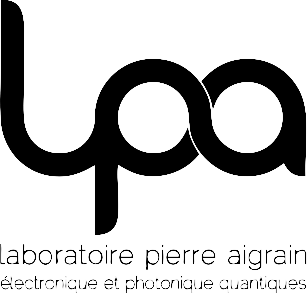
\includegraphics[height=100px]{Images/logo_lpa.png}
\end{flushright}

\vspace*{0.5cm}
\begin{center}
\rule{\linewidth}{0.5mm}\\[0.4cm]
{\huge{\bfseries Rapport de Stage d'Application}\\[0.4cm]
Mise en place d'une expérience à très basse température et étude d'effets quantiques dans des systèmes nanométriques\\[0.4cm]}
\rule{\linewidth}{0.5mm}\\[0.5cm]

\LARGE{\textsc{Félix Piédallu}}\\[0.7cm]
\large{\textsc{Filière PNS 2014-2015}}\\[2cm]

\Large{Au sein de l'équipe HQC}\\[1cm]

\includegraphics[width=0.4\textwidth]{Images/logo_HQC.pdf}\\[1cm]

\large{Sous la direction de Takis \textsc{Kontos} et Laure \textsc{Bruhat}}\\[2cm]


\end{center}
\end{titlepage}

\tableofcontents        % Table des matières avec liens, générée automatiquement.
\newpage
\pagenumbering{arabic}  % Numérotation de retour !


% Remerciements
\vspace*{\stretch{1}}
\begin{center}
\textsc{\Large Remerciements}
\\
\vspace{0.5cm}
Je tiens à remercier Takis Kontos et Laure Bruhat pour m'avoir accueilli au sein de l'équipe HQC, ainsi que pour m'avoir encadré durant ce stage. De plus, je souhaite remercier l'ensemble des membres de l'équipe avec lesquels j'ai pu échanger sur leurs projets de recherche. Enfin, je souhaite remercier Phelma Grenoble-INP pour m'avoir donné l'opportunité de réaliser ce stage.
\end{center}
\vspace*{\stretch{3}}

\chapter*{Hybrid Quantum Circuits}
L'équipe HQC fait partie du Laboratoire Pierre Aigrain, le laboratoire de l'ENS Ulm spécialisé dans la physique de la matière condensée et la physique mésoscopique.

Basé à Paris, il regroupe autour de Takis Kontos et Audrey Cottet plusieurs doctorants : Matthieu Baillergeau, Matthieu Desjardins, Matthieu Dartiailh et Laure Bruhat, avec qui j'ai essentiellement travaillé durant mon stage.

Les sujets de recherche sont essentiellement concentrés autour du transport quantique dans des nanotubes de carbone.
%TODO remplir ce paragraphe

\chapter*{Introduction} % Contexte du stage
\addcontentsline{toc}{chapter}{Introduction}

Laure Bruhat a entamé depuis plus de deux ans une thèse portant notamment sur la séparation des paires de Cooper intriquées dans une cavité micro-ondes et le transport quantique. Pour ce faire, elle a mis en place une expérience dans un cryostat à dilution sèche, fourni par CryoConcept.
\newline
\begin{figure}[h]
    \begin{center}
        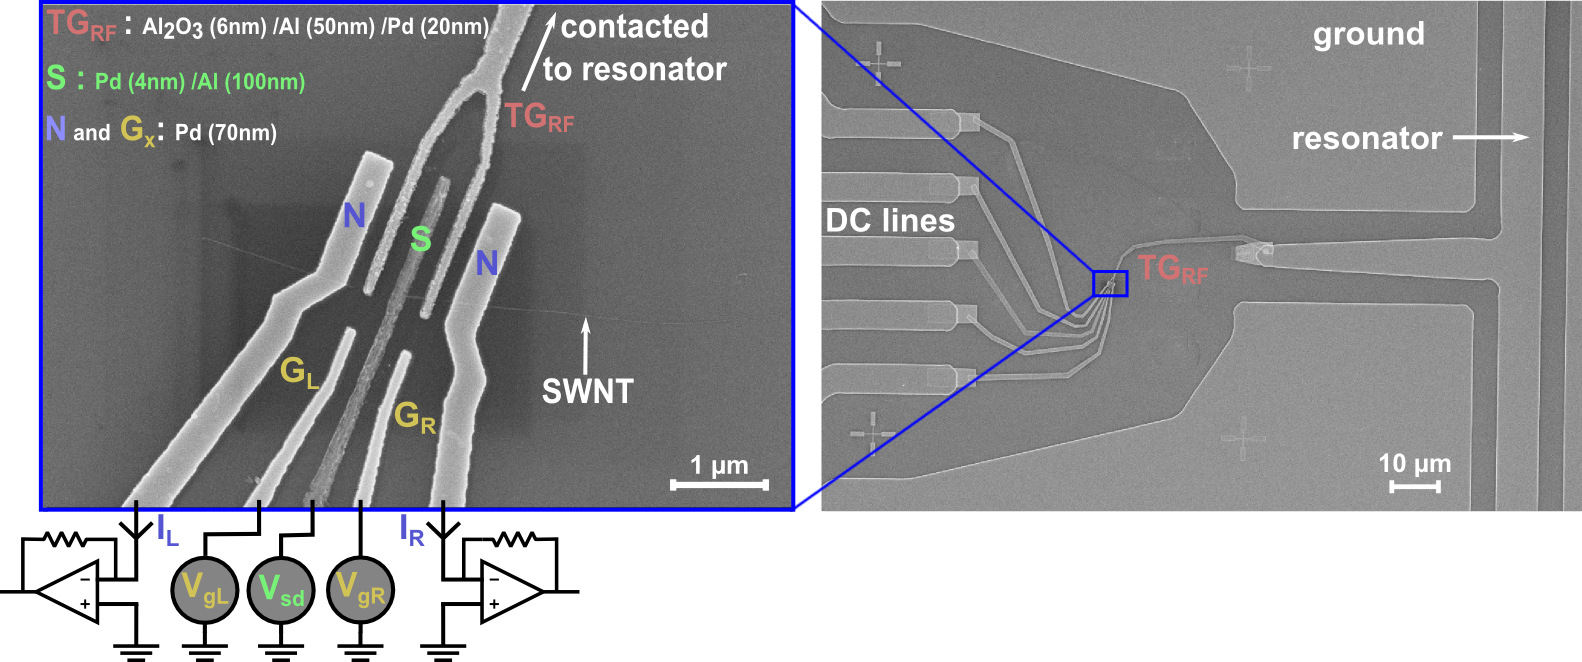
\includegraphics[width=\textwidth]{Images/Expe_photo.jpg}
        \caption*{Photo du séparateur de paires de Cooper à nanofil de carbone}
        \label{fig:}
    \end{center}
\end{figure}


Ce cryostat étant "spacieux", Takis Kontos et Laure Bruhat ont décidé d'y rajouter une expérience. Celle-ci serait placée au sein d'un champ magnétique, généré par une bobine installée dans le cryostat. Cette expérience pourra donc permettre d'étudier l'influence du champ magnétique (quelques 100mT) sur la séparation des paires de Cooper.

J'interviens donc pour aider l'équipe à câbler le cryostat pour cette seconde expérience ainsi que pour les tests du cryostat après la mise en place de la bobine.


\chapter{L'expérience}

\section{Interaction d'électrons et de photons dans un nanotube de carbone}
\subsection{Un milieu 1D (nanotube)}

\subsection{Une cohérence spatiale (atome artificiel)}
$\rightarrow$ Pas de bruit ambiant $\rightarrow$ cryostat

\subsection{L'interaction Électrons/Rayonnement Gigahertz}
$\rightarrow$ Contrôle excellent du signal envoyé $\rightarrow$ câbles coaxiaux les plus parfaits possibles

\subsection{Quelques exemples d'expériences}
\begin{itemize}
    \item Cooper Pair Splitter
    \item Couplage Champ électrique/Trajectoire/Spin
\end{itemize}

\section{Fabrication des nanotubes de Carbone}

\section{Utilisation du champ magnétique}

\chapter{Le cryostat à dilution}
Afin d'accéder à des températures de l'ordre que la dizaine de milliKelvins, l'équipe a décidé d'utiliser un cryostat à dilution sec.
\section{Principe d'un cryostat à dilution}
\begin{figure}[h]
  \begin{center}
    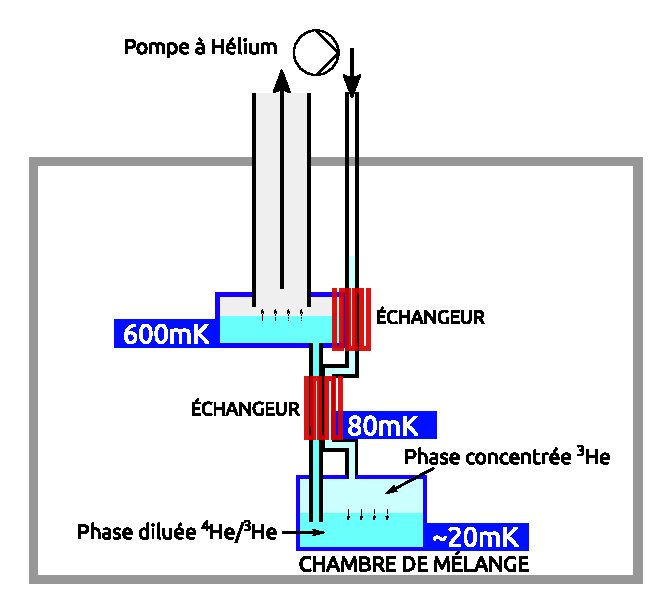
\includegraphics[width=0.6\textwidth]{Images/Cryostat_Schema.pdf}
    \qquad
    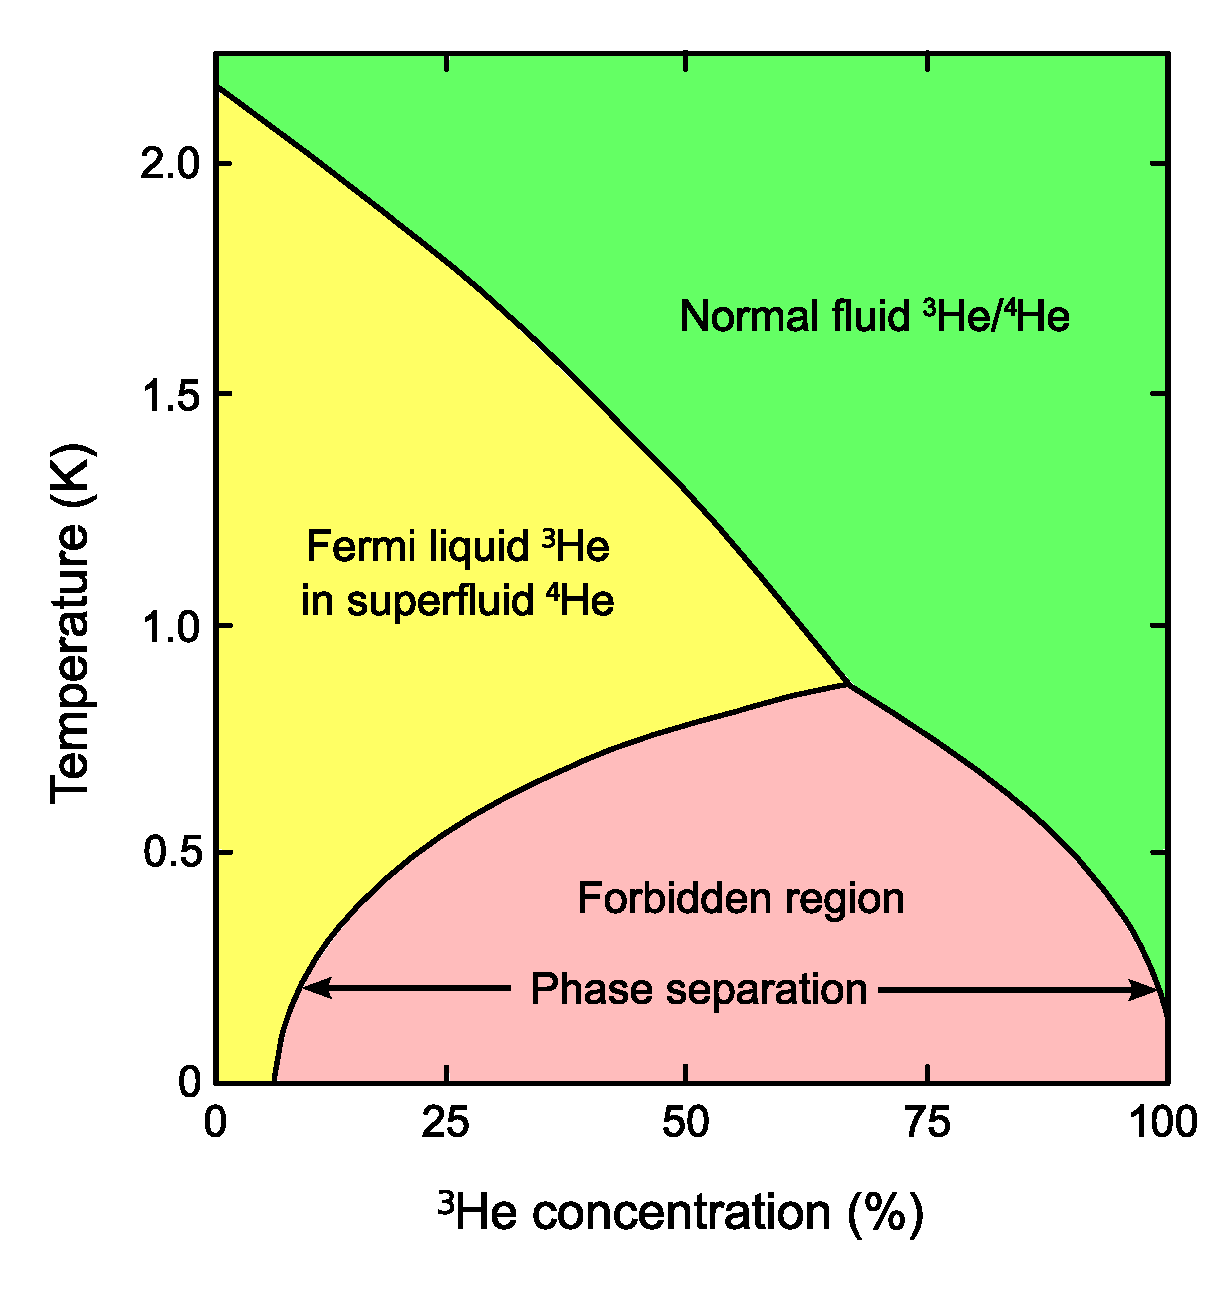
\includegraphics[width=0.33\textwidth]{Images/Helium_phase_diagram.pdf}
    \caption{Schéma du cryostat à dilution et diagramme de phase du mélange d'Hélium}
  \end{center}
\end{figure}
Le cryostat à dilution est basé sur certaines propriétés du mélange des isotopes d'Hélium \HeT et \HeQ.
\newline

Prenons un mélange équilibré liquide (donc pré-refroidi à 1K, nous verrons cela plus tard) ; l'\HeQ étant le plus lourd, il tombe au fond et l'\HeT flotte au-dessus.

Ensuite, du point de vue des interactions quantiques dans chacun des liquides, on remarque que les interactions pour l'atome d'\HeT sont plus faibles que pour l'\HeQ : les premiers vont descendre dans la phase \HeQ, mais pas l'inverse.
\newline
On se trouve donc en présence de deux phases : celle, plus légère, d'\HeT pur, et celle de mélange \HeT/\HeQ.
Enfin, les atomes d'\HeT sont des Fermions, et le principe d'exclusion de Pauli s'y applique : la solubilité de l'\HeT dans l'\HeQ sera limitée aux environs de \{6,6\% \HeT, 93.4\% \HeQ\}.
\newline

On se trouve donc en présence de deux phases : celle, plus légère, d'\HeT pur, et celle de mélange \HeT/\HeQ.
\newline

Or la pompe (à température ambiante) impose une pression plus faible dans le still (~10Pa) qu'en entrée du circuit. L'\HeT va donc passer de la phase pure à la phase de mélange. Mais cette réaction de dilution est endothermique, ce qui fourni la puissance calorifique au cryostat.
%TODO traduction de still

Le mélange pompé va monter dans le still, où seul l'\HeT va s'évaporer. En effet, celui-ci a une pression partielle bien plus élevée que l'\HeQ, il va donc s'évaporer en premier par pression osmotique.

Il va être réinjecté par la pompe pour réaugmenter la pression dans la phase pure d'\HeT et recommencer le cycle.
\newline

Les échangeurs thermiques permettent à l'\HeT réinjecté d'être remis à basse température pour ne pas réchauffer l'ensemble du cryostat. Cela permet aussi d'augmenter la température dans le still et permettre à l'\HeT de s'évaporer plus facilement.

\section{Cryostat sec : Principe du tube à gaz pulsé}
Le mélange doit être pré-refroidi avant d'être injecté dans le cryostat.\newline
La plupart des cryostats utilisent un bain d'azote liquide à 77K qui permet aussi de nettoyer le mélange des impuretés, un bain d'\HeQ liquide à 4,2K, puis un bain d'\HeQ à faible pression à 1K (diminuer la pression de l'\HeQ permet d'abaisser son point de condensation).

Ces derniers bains nécessitant un apport d'\HeQ, il peuvent être remplacé par un tube à gaz pulsé, d'où l'appellation de cryostat sec (mis à part le bain d'azote liquide qui est à l'extérieur du cryostat).

\begin{figure}[h]
    \begin{center}
        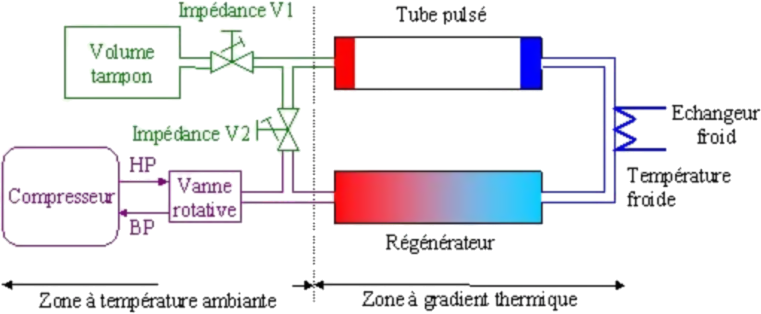
\includegraphics[width=0.75\textwidth]{Images/Cryostat_PulseTube_Schema.png}
        \caption{Schéma du tube à gaz pulsé}
    \end{center}
\end{figure}

\begin{figure}[h]
    \begin{center}
        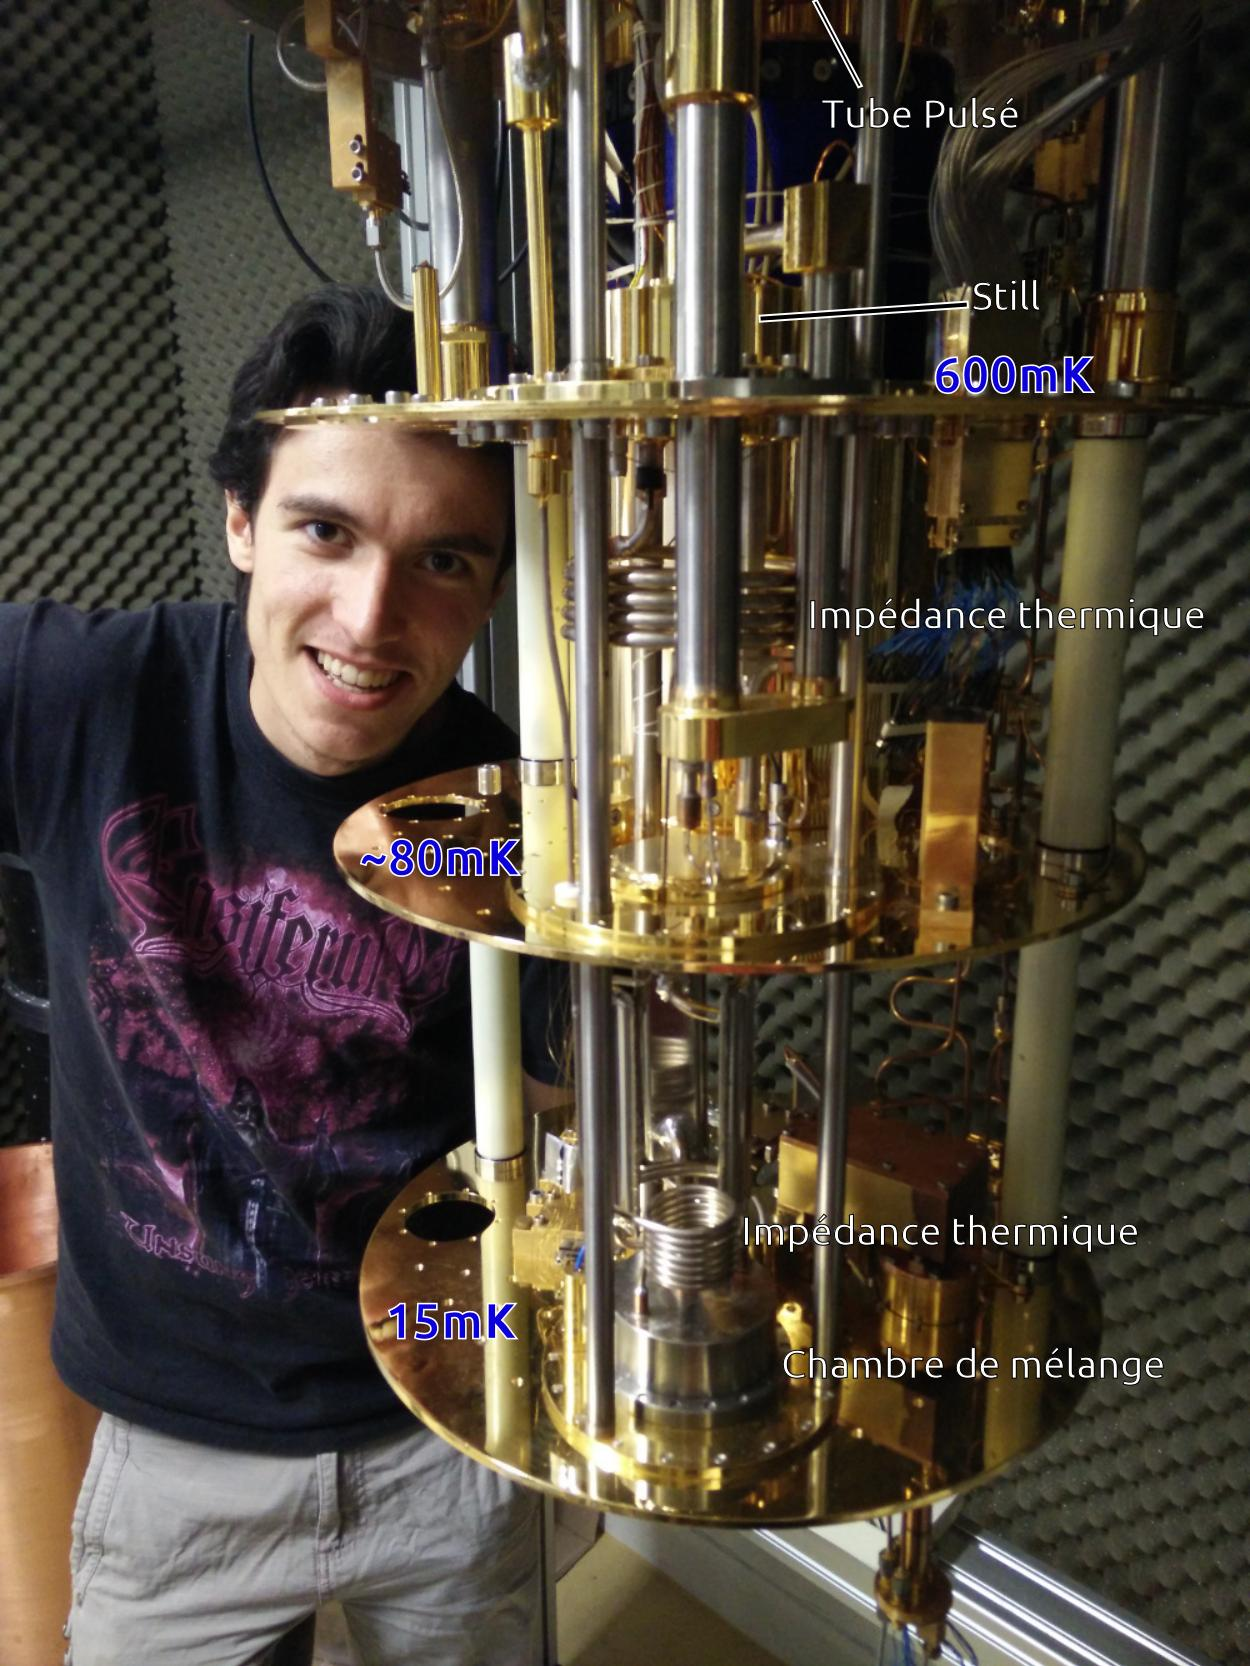
\includegraphics[width=0.75\textwidth]{Images/PhotoCryostat}
        \caption{Organisation du cryostat à dilution sèche}
    \end{center}
\end{figure}


\chapter{Le câblage DC et RF}
\begin{figure}[h]
    \begin{center}
        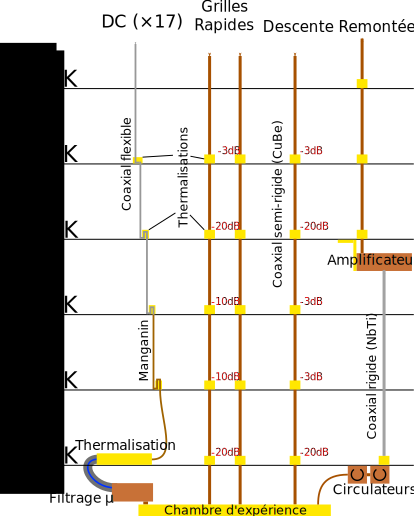
\includegraphics[width=0.7\textwidth]{Images/Cablage_schema}
        \caption{}
        \label{fig:}
    \end{center}
\end{figure}

Le câblage du cryostat consiste en deux parties : 
\paragraph*{Les câbles DC : } ils véhiculent les signaux continus. Au nombre de 17, ils sont thermalisés à chaque étage pour limiter le bruit thermique.
\paragraph*{Les câbles coaxiaux : } les deux grilles rapides, le signal d'entrée et le signal de sortie. Ils font l'objet de beaucoup d'attention, afin d'avoir les meilleures mesures possibles.


\section{Choix des matériaux}
Parlons tout d'abord des câbles de descente. Ceux-ci véhiculent le bruit thermique d'étage en étage, ce que nous voulons limiter au maximum.

Nous ferons donc le choix de câbles atténuant le signal afin de limiter l'apport de bruit. Ceci permet de plus de limiter les ponts thermiques entre étages dûs à la conductivité des câbles.
\newline

Les câbles DC sont alors :
\begin{itemize}
    \item des câbles coaxiaux entre 300K et 800mK, peu résistifs (le signal est suffisant pour avoir un bon rapport signal/bruit)
    \item des câbles de Manganin, très résistif, jusqu'à 20mK (l'étage le plus froid)
    \item des câbles peu résistifs jusqu'à la chambre d'expérience
\end{itemize}

et les câbles RF de descente sont :
\begin{itemize}
    \item en Cuivre-Béryllium, thermalisé à chaque étage, jusqu'à 20mK. Le CuBe est beaucoup plus résistif que le Cuivre.
    \item en Cuivre jusqu'à la chambre d'expérience
\end{itemize}

Les câbles sont cintrés en "U" entre chaque étage, afin de limiter les radiations au maximum. Ceci permet de plus d'avoir une certaine souplesse dans les câbles pour les connecter sans trop de difficultés.

\paragraph*{Pour le câble de remontée,} on raisonne différemment : il faut atténuer le signal le moins possible, jusqu'à l'amplificateur haute fréquence qui est situé à 4K (sa température nominale de fonctionnement). Un câble rigide de Niobium-Titane est alors utilisé.

Afin de limiter le "retour" de signal de l'amplificateur par ce câble, on thermalise deux circulateurs à 20mK. On utilise des câbles de Cuivre pour les connexions avec la chambre d'expérience.

%\section{Principe des câbles coaxiaux}
\section{Thermalisation électronique}
Une grande partie du bruit provient de la température électronique. Si les câbles ne sont pas bien thermalisés, elle n'est pas assez faible et on risque même de ne mesurer qu'un bruit à 300K.

Les câbles coaxiaux sont thermalisés à chaque étage par des pinces, reliées par des câbles de cuivre jusqu'aux platines du cryostat. L'ensemble des pièces est bien sûr doré pour avoir les meilleurs contacts thermiques possibles ; on utilise aussi de l'Apiezon N, une graisse cryogénique pour boucher les pores des parois en contact, à l'instar de la pâte thermique de nos processeurs.
\newline

Les câbles DC sont thermalisés à chaque étage par des pinces dorées grâce à de la Stycast. Cette époxy permet une très bonne thermalisation des câbles fins aux presses dorées et montées sur les platines du cryostat.

Une thermalisation s'effectue aussi au niveau du boîtier de thermalisation où les câbles font des méandres pour assurer une bonne thermalisation électronique.

\section{Filtrage des lignes DC}
En plus de la thermalisation, les lignes DC sont filtrées à l'étage 20mK. Un premier filtrage est effectué dans le boîtier de thermalisation à l'aide de deux filtres Passe-Bas RC consécutifs.

Un second filtrage est effectué grâce à l'Eccosorb. Cette résine composite à base d'époxy (même fabricant que la Stycast, mêmes solutions) absorbe très efficacement les micro-ondes résultant du bruit électronique.

Il a donc fallu mettre en place un petit boîtier, dans lequel nous faisons passer 17 câbles bleus de 80cm, compartimenté pour que l'Eccosorb n'abîme pas les prises lors du durcissement et des cycles de refroidissement. J'ai donc décidé de dessiner des séparations qui ont été imprimées en 3D en PLA. En effet ce matériau, bien que très commun pour l'impression 3D, s'est avérée utilisable en ultra-vide et à des températures très basses.


\section{Fabrication des câbles coaxiaux}
Comme je l'ai précisé plus haut, les signaux RF sont véhiculés par des câbles coaxiaux semi-rigides.

J'ai donc procédé intégralement à la fabrication et la caractérisation de ces câbles.

La moindre imperfection des câbles coaxiaux se ressent fortement sur leur atténuation -- nous verrons cela plus tard -- , il faut donc les manier et les cintrer en faisant attention à ne pas les tordre.

\paragraph*{Dénudage} Il faut dénuder quelques millimètres du câble pour souder la pin sur l’âme du
câble coaxial. On utilisera le support 21B ainsi que la petite scie. Il faut aller doucement
sans appuyer, jusqu’à ce qu’on sente que c’est "lisse".
\begin{figure}[h]
    \begin{center}
        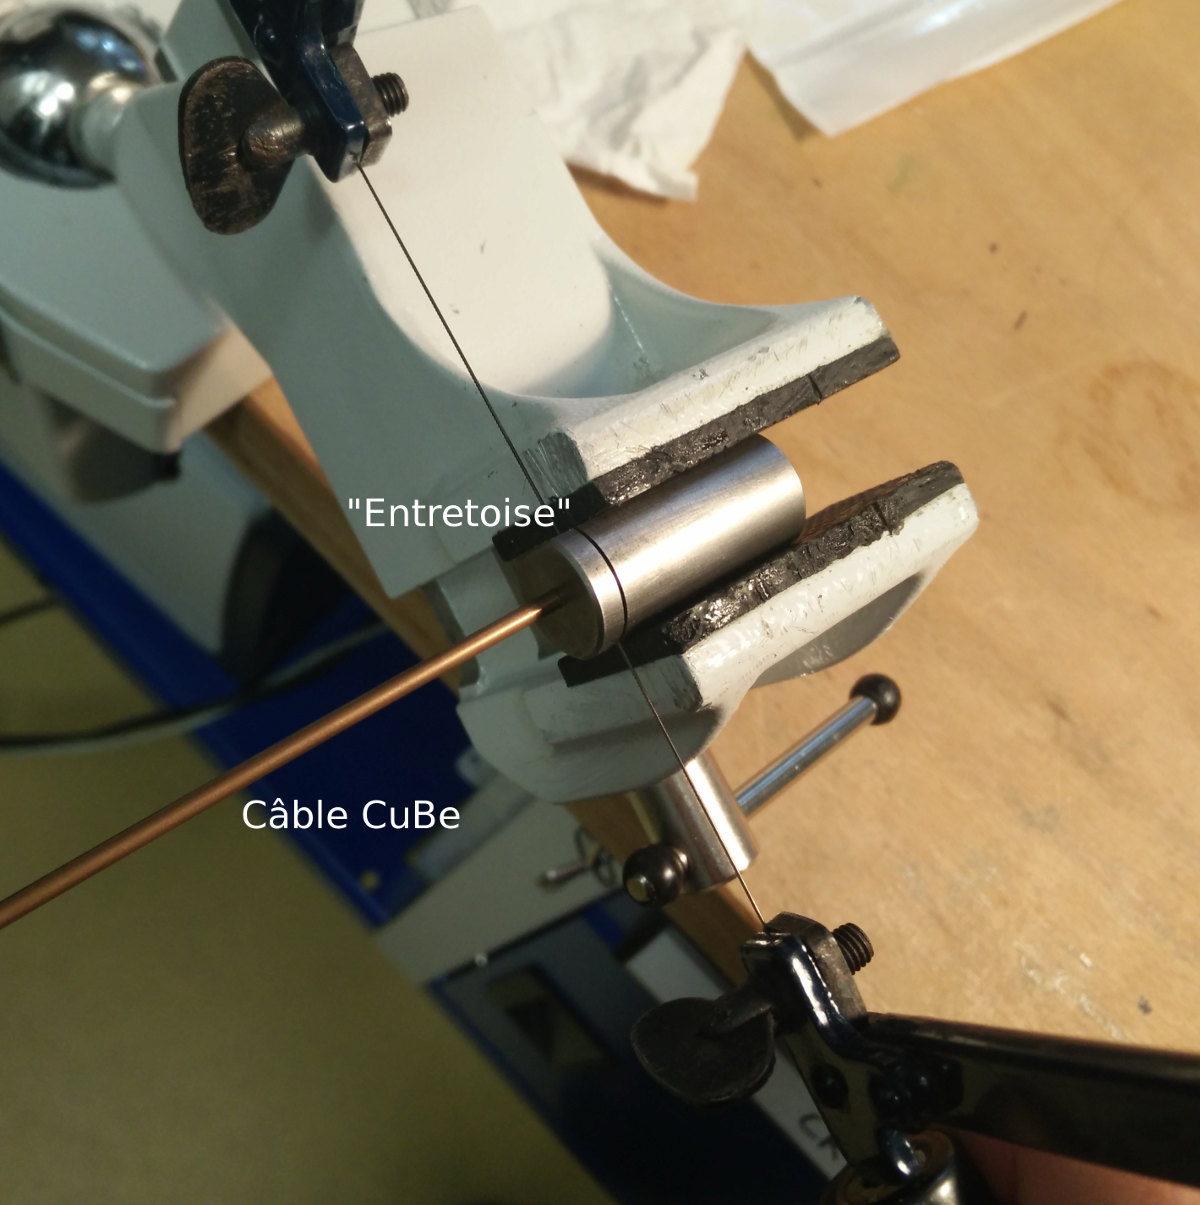
\includegraphics[height=0.48\textwidth]{Images/Coax/1}
        \quad
        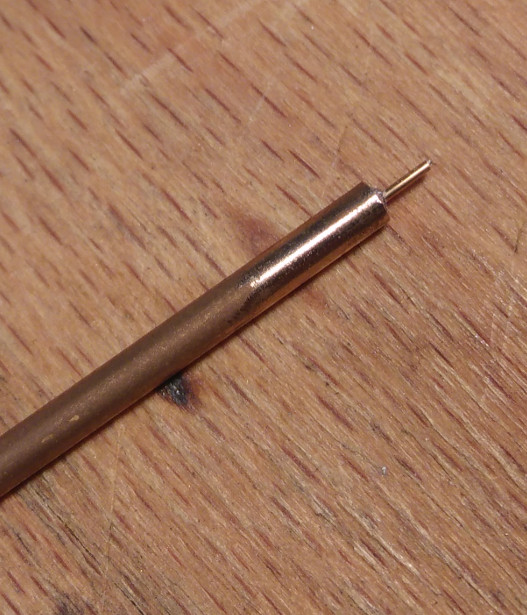
\includegraphics[height=0.48\textwidth]{Images/Coax/2}
        \caption{Dénudage d'un câble coaxial}
        \label{fig:}
    \end{center}
\end{figure}

\paragraph*{Soudure de la pin centrale} On fixe la pin sur l’âme du câble, puis on serre le tout en
place avec la pièce W60 Il ne faut pas oublier l’entretoise W56 entre la pin et l’isolant
encore en place.
Pour souder il suffit de chauffer l’extérieur de la pin tout en positionnant le fil d’étain sur
le trou sur le bord de la pin.
\begin{figure}[h]
    \begin{center}
        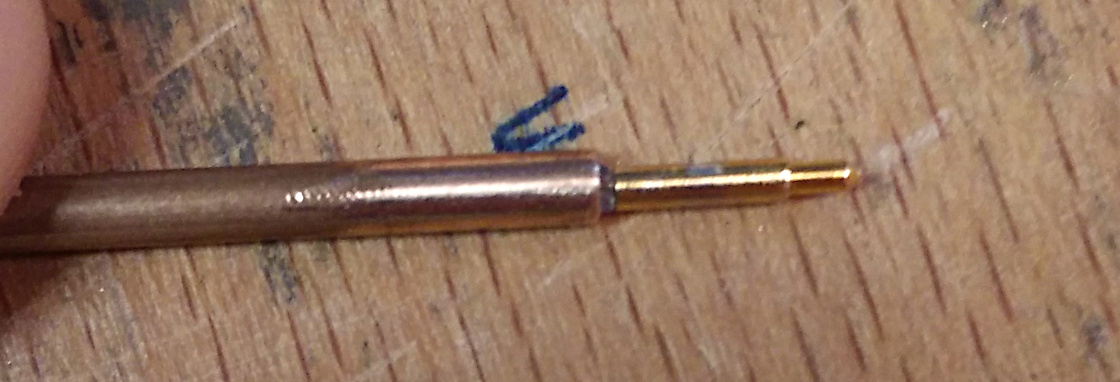
\includegraphics[width=0.60\textwidth]{Images/Coax/3}
        \caption{Pin centrale soudée sur le câble}
        \label{fig:}
    \end{center}
\end{figure}

\paragraph*{Soudure de la prise extérieur} On fixe sur la prise mâle une prise femelle factice W14M
(81) qui permet de positionner comme il faut la prise. Comme à l’étape précédente on
serre le tout en place.
Le plus efficace est de faire un tortillon d’étain au-dessus de la prise, que l’on chauffe. En
étant un peu patient l’étain va fondre et rentrer naturellement dans la prise.
\begin{figure}[h]
    \begin{center}
        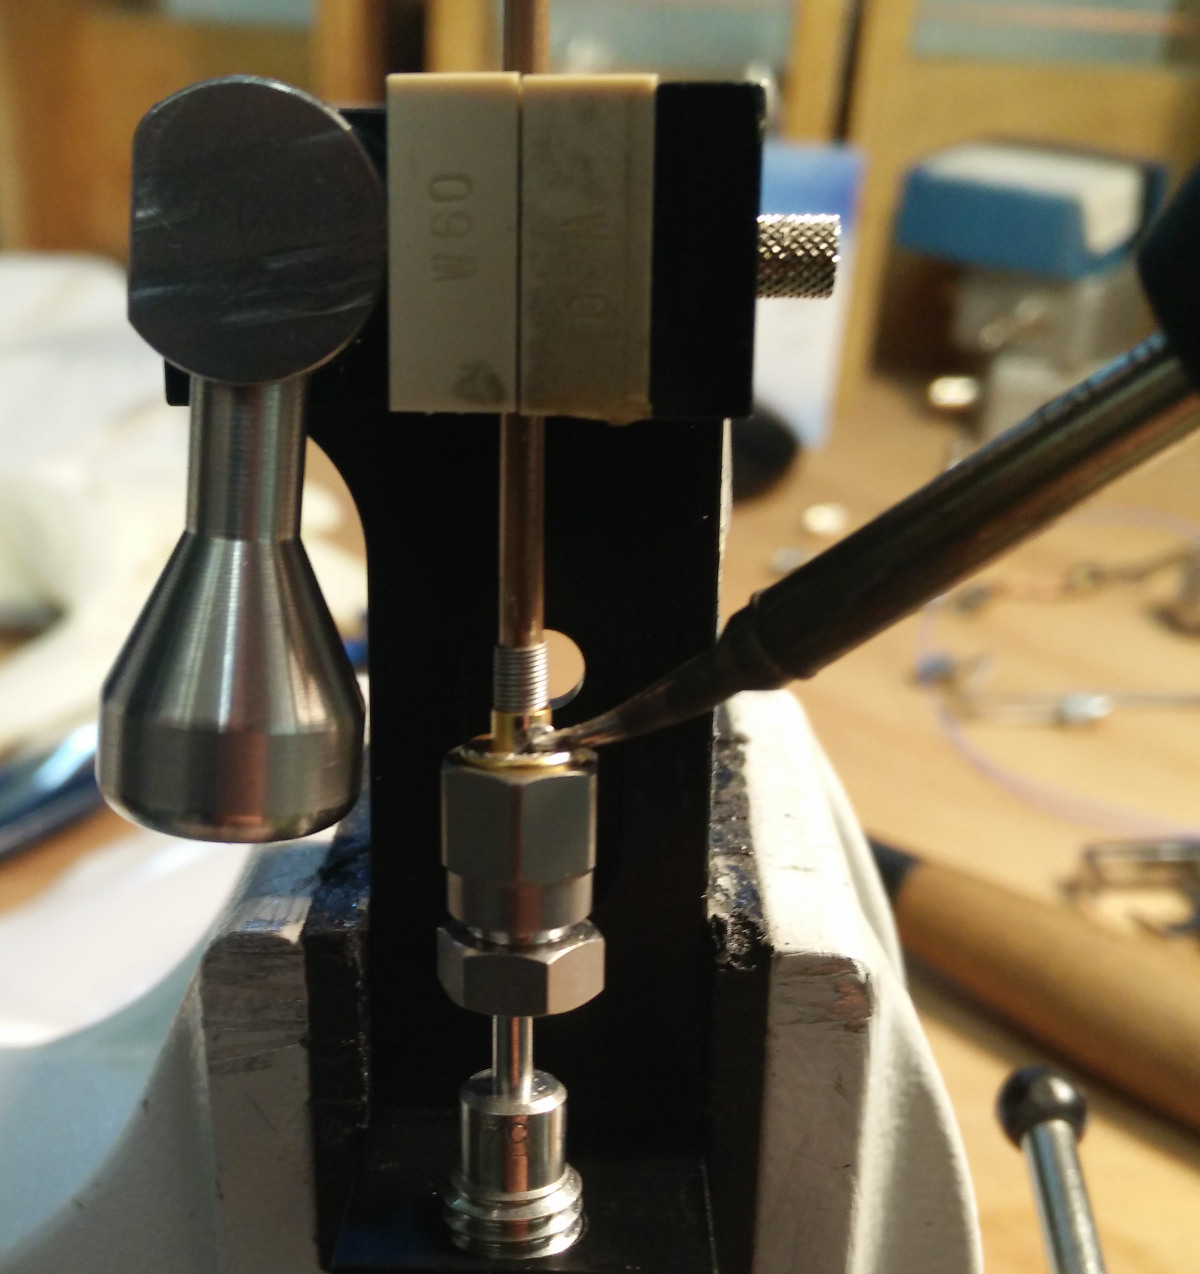
\includegraphics[height=0.48\textwidth]{Images/Coax/4}
        \quad
        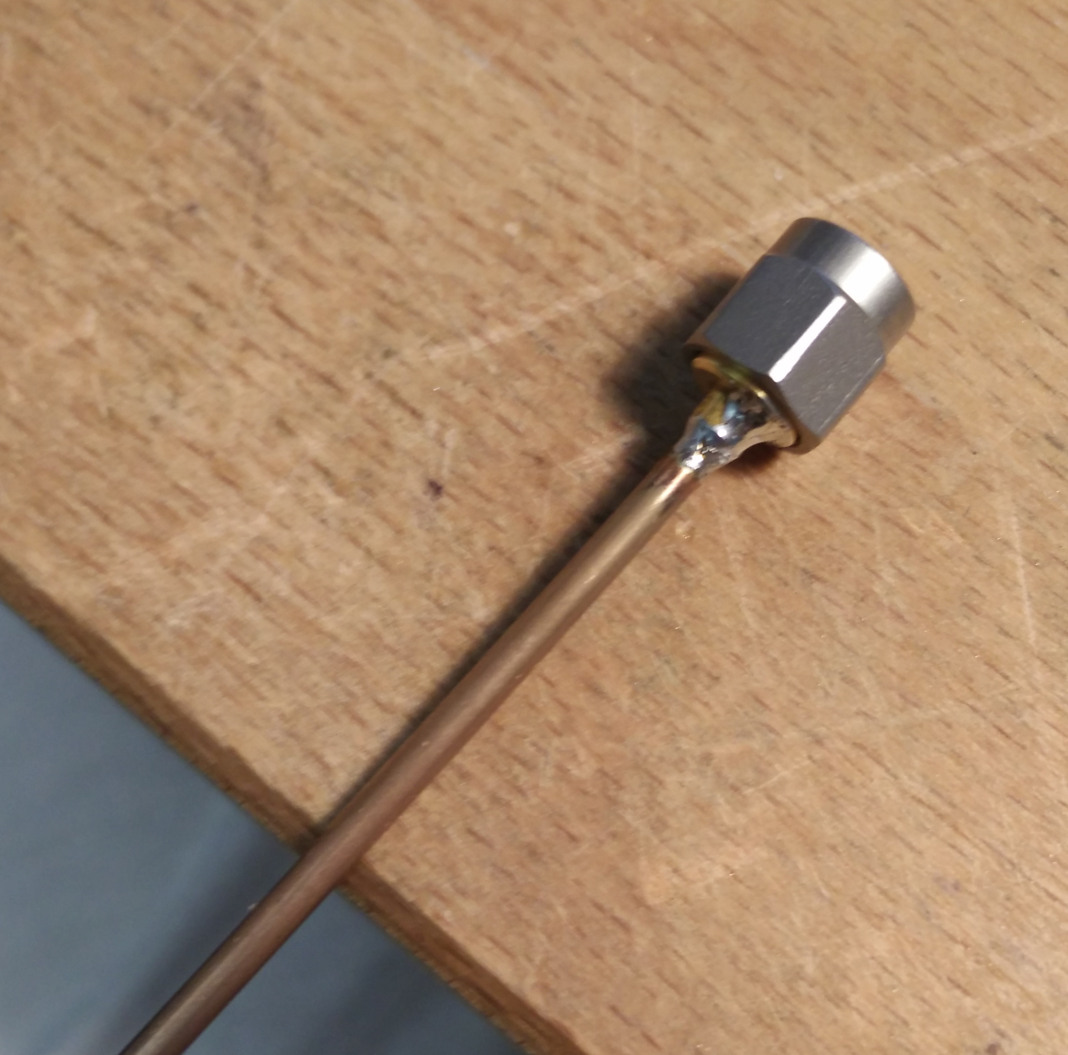
\includegraphics[height=0.48\textwidth]{Images/Coax/5}
        \caption{Soudure de la prise extérieure}
        \label{fig:}
    \end{center}
\end{figure}

\paragraph*{Fixation de l’isolant}  La dernière étape est de mettre l’isolant entre la prise et la pin. on
utilise la pièce W52 (W53) que l’on serre à la clé dynamométrique. On place l’isolant à
l’intérieur, et on pousse d’un coup avec la pièce complémentaire.
Mesure du câble nécessaire Maintenant il faut prendre la dimension de câble à couper.
Sur le montage il faut prendre la dimension entre les deux{}
\begin{figure}[h]
    \begin{center}
        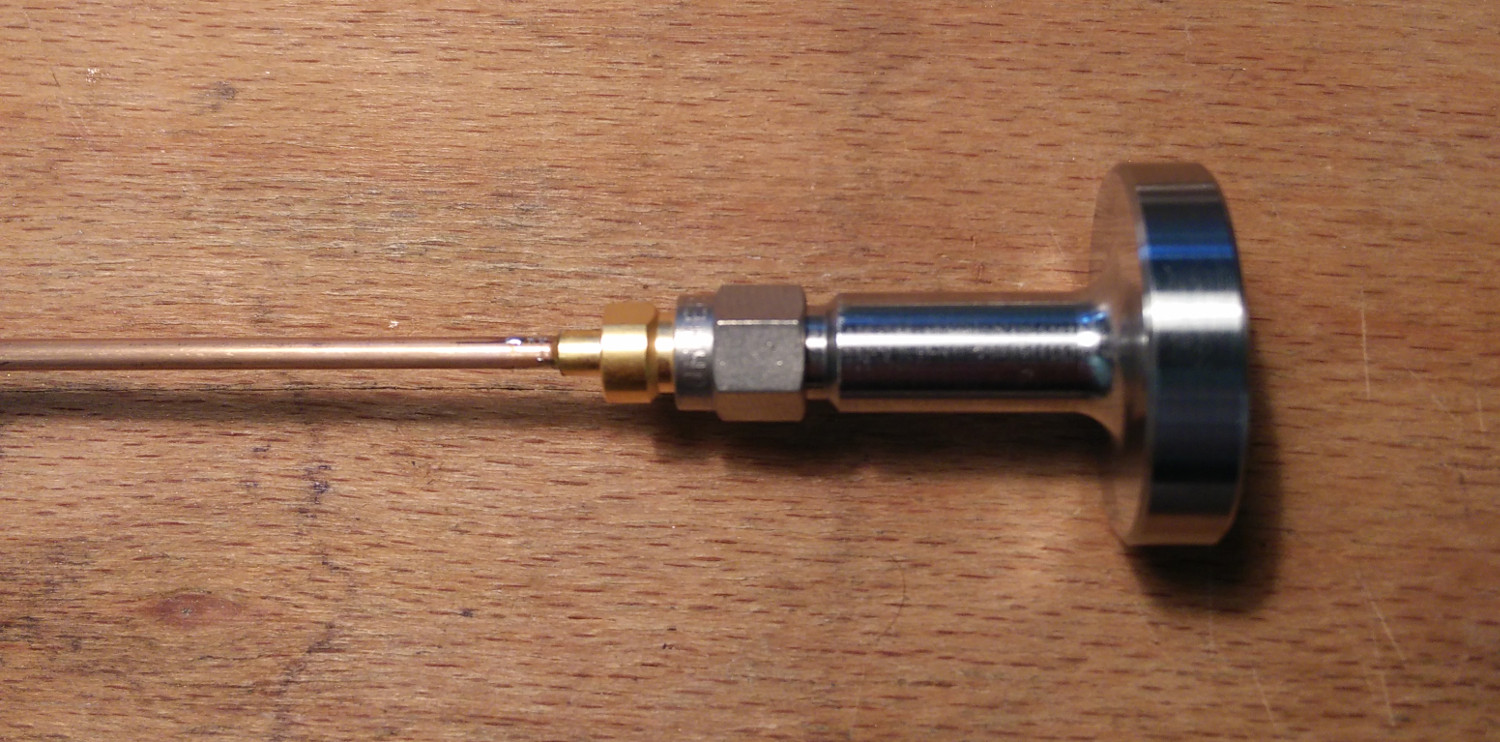
\includegraphics[width=0.60\textwidth]{Images/Coax/6}
        \caption{Fixation de l’isolant}
        \label{fig:}
    \end{center}
\end{figure}

\section{Caractérisation des câbles coaxiaux}


\chapter{Les résultats de l'expérience (avant et/ou après câblage)}

\chapter{Bilan}
\section{Guide de câblage, d'utilisation du VNA,…}
\chapter*{Conclusion}
%\input{6.Conclusion}

\bibliographystyle{unsrt}
\bibliography{bibliographie}
\end{document}
